% ****** Start of file aipsamp.tex ******
%
%   This file is part of the AIP files in the AIP distribution for REVTeX 4.
%   Version 4.1 of REVTeX, October 2009
%
%   Copyright (c) 2009 American Institute of Physics.
%
%   See the AIP README file for restrictions and more information.
%
% TeX'ing this file requires that you have AMS-LaTeX 2.0 installed
% as well as the rest of the prerequisites for REVTeX 4.1
%
% It also requires running BibTeX. The commands are as follows:
%
%  1)  latex  aipsamp
%  2)  bibtex aipsamp
%  3)  latex  aipsamp
%  4)  latex  aipsamp
%
% Use this file as a source of example code for your aip document.
% Use the file aiptemplate.tex as a template for your document.
\documentclass[%
 aip,
 jmp,
 amsmath,
 amssymb,
%preprint,%
 reprint,%
%author-year,%
%author-numerical,%
 numerical,
 longbibliography,
]{revtex4-1}

\usepackage{graphicx}% Include figure files
\graphicspath{{images/}}
\usepackage{dcolumn}% Align table columns on decimal point
\usepackage{bm}% bold math
\usepackage{url}
\usepackage{float}
\usepackage{silence}
\usepackage{tabularx}
\usepackage{verbatimbox}
\WarningFilter{revtex4-1}{Repair the float}
%\usepackage[mathlines]{lineno}% Enable numbering of text and display math
%\linenumbers\relax % Commence numbering lines

\begin{document}

%\preprint{AIP/123-QED}

\title[Laboratory 7]{Latches and Level Conditioners} % Force line breaks with \\

\author{Kevin "Yama" Keyser}
 \email{kk8r8@mail.umck.edu}
\affiliation{ 
	University of Missouri-Kansas City
	%\\This line break forced with \textbackslash\textbackslash
}%

%\date{\today}% It is always \today, today,
             %  but any date may be explicitly specified

\begin{abstract}

In Laboratory 7, we extend our introduction to truth tables and logic gates,
and expand these ideas with our first flip-flop. Specifically a Set-Reset, or
SR flip-flop. We will also construct a schmitt trigger using a comparator Op-Amp,
and finally implement a 555 timer in a circuit.

\end{abstract}

%\keywords{Operational Amplifier}%Use showkeys class option if keyword
                              %display desired
\maketitle

%\begin{quotation}
%The ``lead paragraph'' is encapsulated with the \LaTeX\ 
%\verb+quotation+ environment and is formatted as a single paragraph before the first section heading. 
%(The \verb+quotation+ environment reverts to its usual meaning after the first sectioning command.) 
%Note that numbered references are allowed in the lead paragraph.
%
%The lead paragraph will only be found in an article being prepared for the journal \textit{Chaos}.
%\end{quotation}

\section{Background}

Laboratory 7 bring together (in an abstracted manner) everything we've done up until now. The 555
timer when deconstructed, much like the Op-Amp, is a collection of of Op-Amps, resistors, a switch,
flip-flop, and buffer (which we haven't used) to create a circuit that gives us specific square wave
timing. In this one chip is everything we've used up until now. 

\section{Procedure}

The procedures for Laboratory 7 will be attached as a separate sheet of paper to the back
of the laboratory write up.

\section{Presentation of Data}

	\subsection{7-1: Building a "Set-Reset" Latch with NAND gates}
	
	\begin{tabularx}{0.45\textwidth}[t]{| X | X | X | X |}
	\hline
	\multicolumn{4}{|c|}{NAND SR Truth Table}\\
	\hline	
	\multicolumn{1}{|c|}{S} & \multicolumn{1}{c|}{R} & \multicolumn{1}{c|}{Q} & \multicolumn{1}{c|}{Q'}\\ \hline
	\hline
	1 & 0 & 0 & 1 \\ \hline
	1 & 1 & 0 & 1 \\ \hline
	0 & 1 & 1 & 0 \\ \hline
	1 & 1 & 1 & 0 \\ \hline
	\end{tabularx}

	\subsection{7-2: Building a "Set-Reset" Latch with NOR gates}
	
	\begin{tabularx}{0.45\textwidth}[t]{| X | X | X | X |}
	\hline
	\multicolumn{4}{|c|}{NOR SR Truth Table}\\
	\hline	
	\multicolumn{1}{|c|}{S} & \multicolumn{1}{c|}{R} & \multicolumn{1}{c|}{Q} & \multicolumn{1}{c|}{Q'}\\ \hline
	\hline
	1 & 0 & 1 & 0 \\ \hline
	0 & 0 & 1 & 0 \\ \hline
	0 & 1 & 0 & 1 \\ \hline
	0 & 0 & 0 & 1 \\ \hline
	\end{tabularx}
	
	\subsection{7-3: Level Conditioning}
	
	\begin{figure}[H]
	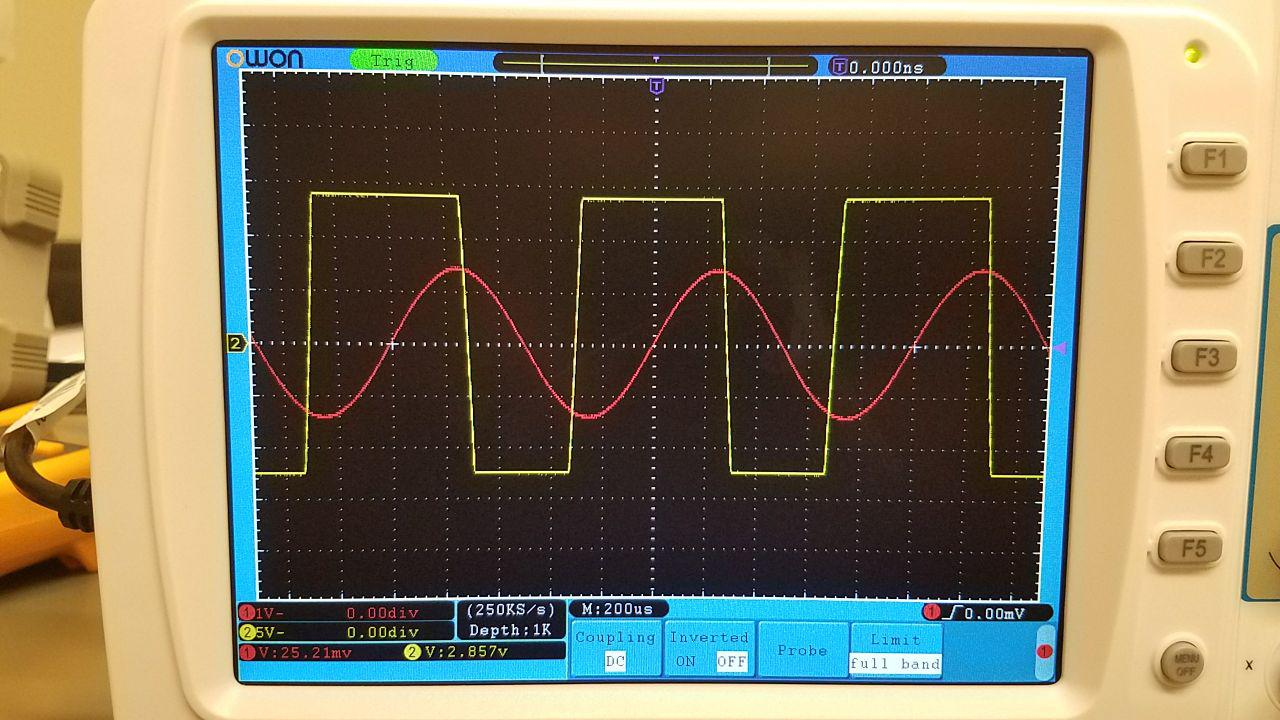
\includegraphics[width=\columnwidth]{73-400Hz.eps}
	\caption{Input and output for Schmidt trigger at 400Hz.}
	\end{figure}
	
	\begin{figure}[H]
	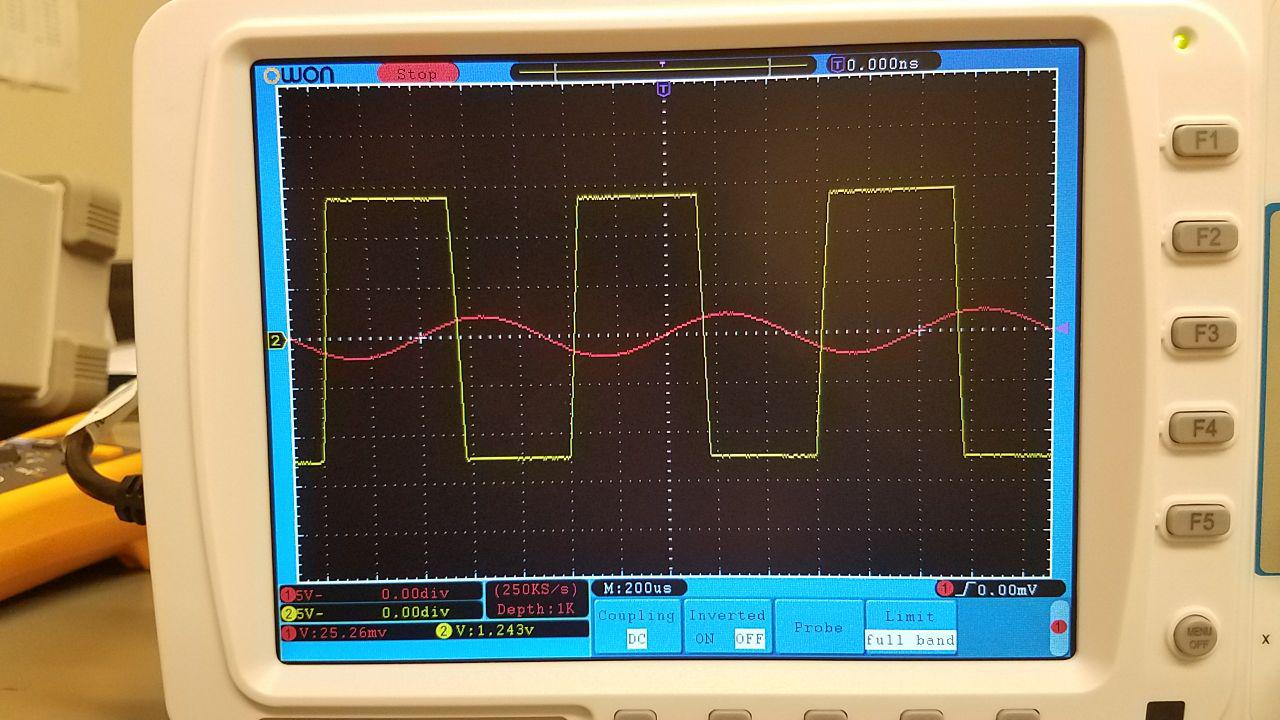
\includegraphics[width=\columnwidth]{73-1kHz.eps}
	\caption{Input and output for Schmidt trigger at 1kHz.}
	\end{figure}
	
	\begin{figure}[H]
	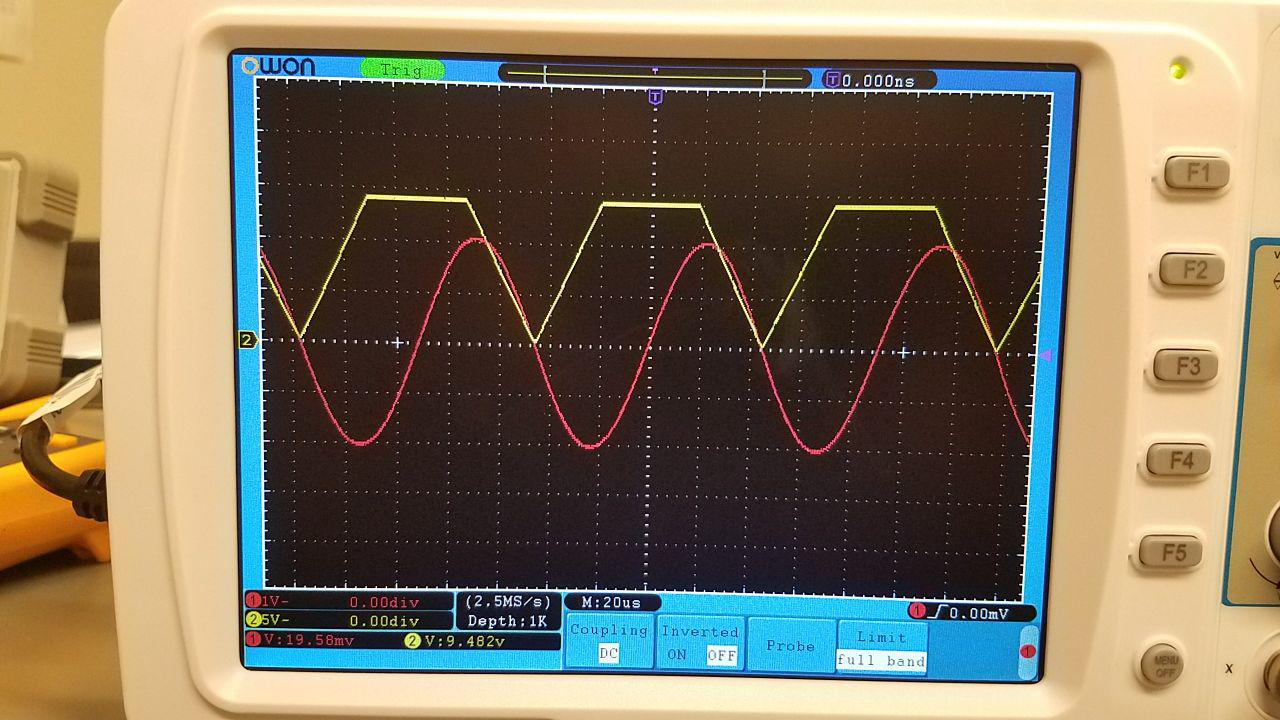
\includegraphics[width=\columnwidth]{73-11kHz.eps}
	\caption{Input and output for Schmidt trigger at 11kHz}
	\end{figure}
	
	\subsection{7-4: 555 Timer Circuit}	
	
	\begin{figure}[H]
	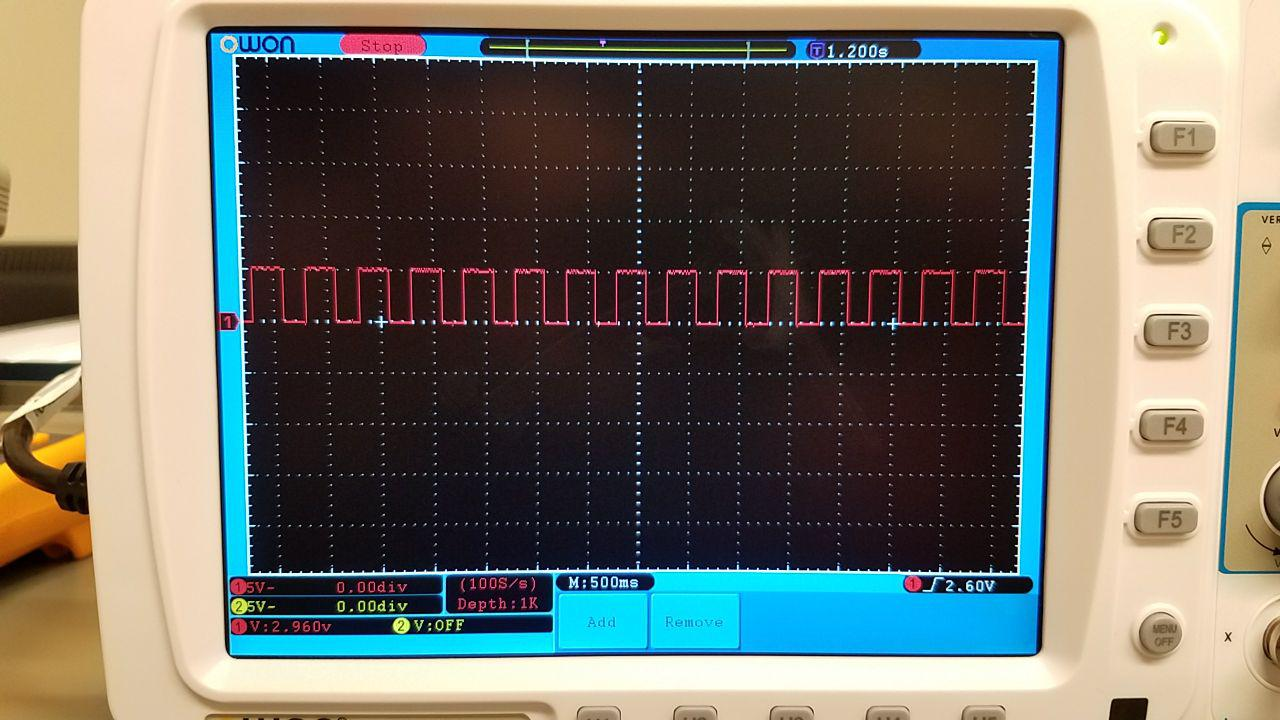
\includegraphics[width=\columnwidth]{74-555.eps}
	\caption{Cycle for 555 timer}
	\end{figure}
	
\section{Discussion}
	
	\subsection{7-1: Building a "Set-Reset" Latch with NAND gates}
	
	When looking at the results of our truth table, and what the intended application of
	our Set-Reset flip-flop is, we can figure out which states Sets and Resets our values.
	We can see that S=1 and R=1 is a two state stable state. It remembers the previous value
	that came before it, so regardless if S was 0 or R was 0, when they're put back to 1, 
	the SR flip-flop will still keep its previous value. Then we can see that the zero value,
	or the off value is what actually triggers our desired effect for this circuit. When
	R is 0, our Q becomes 0, no matter what its previous value was. When S is 0, our Q becomes
	1, no matter what our previous value for Q was. Q' will always output the negation of Q 
	in this circuit.

	\subsection{7-2: Building a "Set-Reset" Latch with NOR gates}
	
	The NOR implementation of the SR flip-flop works more in line with what we would want
	for our logic gates, as it requires less power to keep circuit in our stable state. This
	time, when S=0, R=0, this is our two state stable state. So the previous value of Q is
	preserved. Now, when S is 1, our Q becomes 1. When R is 1, Q becomes 0. Similarly, Q'
	is the negation of Q.
	
	\subsection{7-3: Level Conditioning}
	
	With the Schmidt trigger we were able to find different $V_{pp}$ values for different frequencies
	at which the square wave for our output stabilizes. At 400Hz, we can be at 2.72 $V_{pp}$, where
	for 1kHz we go slightly higher to 2.75 $V_{pp}$. At lower frequencies, this number seems to drop,
	where at higher values for frequency, we stop seeing inversion happen. There is not enough time for
	this transition to happen. At 11kHz, we see our square wave look more trapezoidal, and it no longer
	reaches negative values. Since the default output is +15V in our configuration, it makes sense that
	it requires a high enough, and long enough positive voltage to give us our negative output (since
	we are doing an inverted input). When the frequency goes too high, it can't transition fast enough
	and we get values that no longer can be inverted.
	
	\subsection{7-4: 555 Timer Circuit}	
	
	The formula for time to be a high output is given by $T_H=0.7(R_1+R_2)C$.
	The formula for time to be a low output is given by $T_L=0.7R_2C$. If we have a desired 
	high and low, the best thing to do is to pick a capacitor, plug it into our equation for 
	$T_L$, since we know what our $T_L$ we want, and we get our $R_2$. We can do the same by
	plugging our solved values into the equation for $T_H$, and solve for $R_1$. This is how
	we chose our values for our capacitors, with $C=1\mu F$, $R_1=100k\Omega$, and 
	$R_2=300k\Omega$. This gives us an approximate $T_H=0.3s$, and $T_L=0.2s$. Since the period
	is how much time it takes for a function to get back to where it was, we can add both together
	to get $T=T_H+T_L$, to get a period of 0.5s.
	
\section{Conclusion}

From 7-1 and 7-2, we see how we can construct a Set-Reset Latch, or Flip-Flop as known in the 
Computer Science field. The SR flip-flop is used to set a value and reset a value. This can be
useful for storing values, like we do in RAM. Both versions show that there are separate ways
of implementing an SR flip-flop, and how to read the truth tables (more importantly, how to
predict the truth tables) for each. Though from the writer's point of view, the NOR version
seems more intuitive than the NAND implementation.

Using a 555 timer in addition to the SR flip-flop, we can set a time for how often we want
these values to be update. We can choose how long a clock cycle is with this set up. Though
our 0.5s is not very realistic for any practical use, the implementation of and execution of
our given formula gives us the basic underlying use of the circuitry.

\end{document}